\section{Part III: Nonlinear Dimensionality Reduction (for dataset B)}

Dataset B was partitioned to contain only the digit "3" for parts 1 and 2 of this section. Figure~\ref{fig:fig8} displays all the hand written digits "3" available in the subset. Looking at the images qualitatively, not all "3's" are drawn equally. Images differ with respect to: tilt (either left or right), line weights (thick or thin), width and curvature, to name a few features. 
\begin{figure}[htb]
 \centering
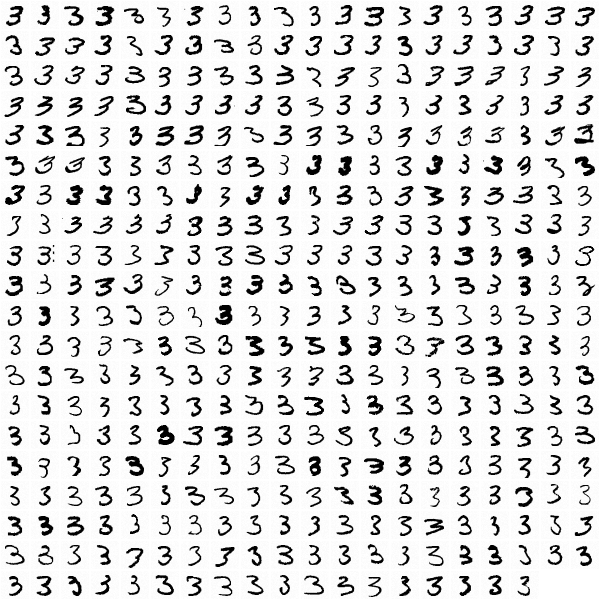
\includegraphics[width=4in]{assignment1/3-0-alldigit3.png}
\caption{\label{fig:fig8}This gives us an idea of the variety of handwriting styles for digit 3 in the dataset}
\end{figure}


\clearpage{}
\subsection{Apply LLE to the images of digit '3' only}
 The reduced structure looks like (fill in )shape. We can see that the digits on the left side towards the center are tilted right, while the digits on the right side are straight with the exception of a few at the top right corner tilted left. And keeping in accordance to the direction of the digits, the digits on the lower right part  have thinner strokes,while the digits at the left and  near the left part  have thicker strokes. Majority of the weird '3's  tend to be near the right center to the lower right  corner. There is a very clear pattern of where the images are placed. 
 LLE did the best in mapping the digits in the reduced dimension.


Figure~\ref{fig:fig9} 
\begin{figure}[htb]
 \centering
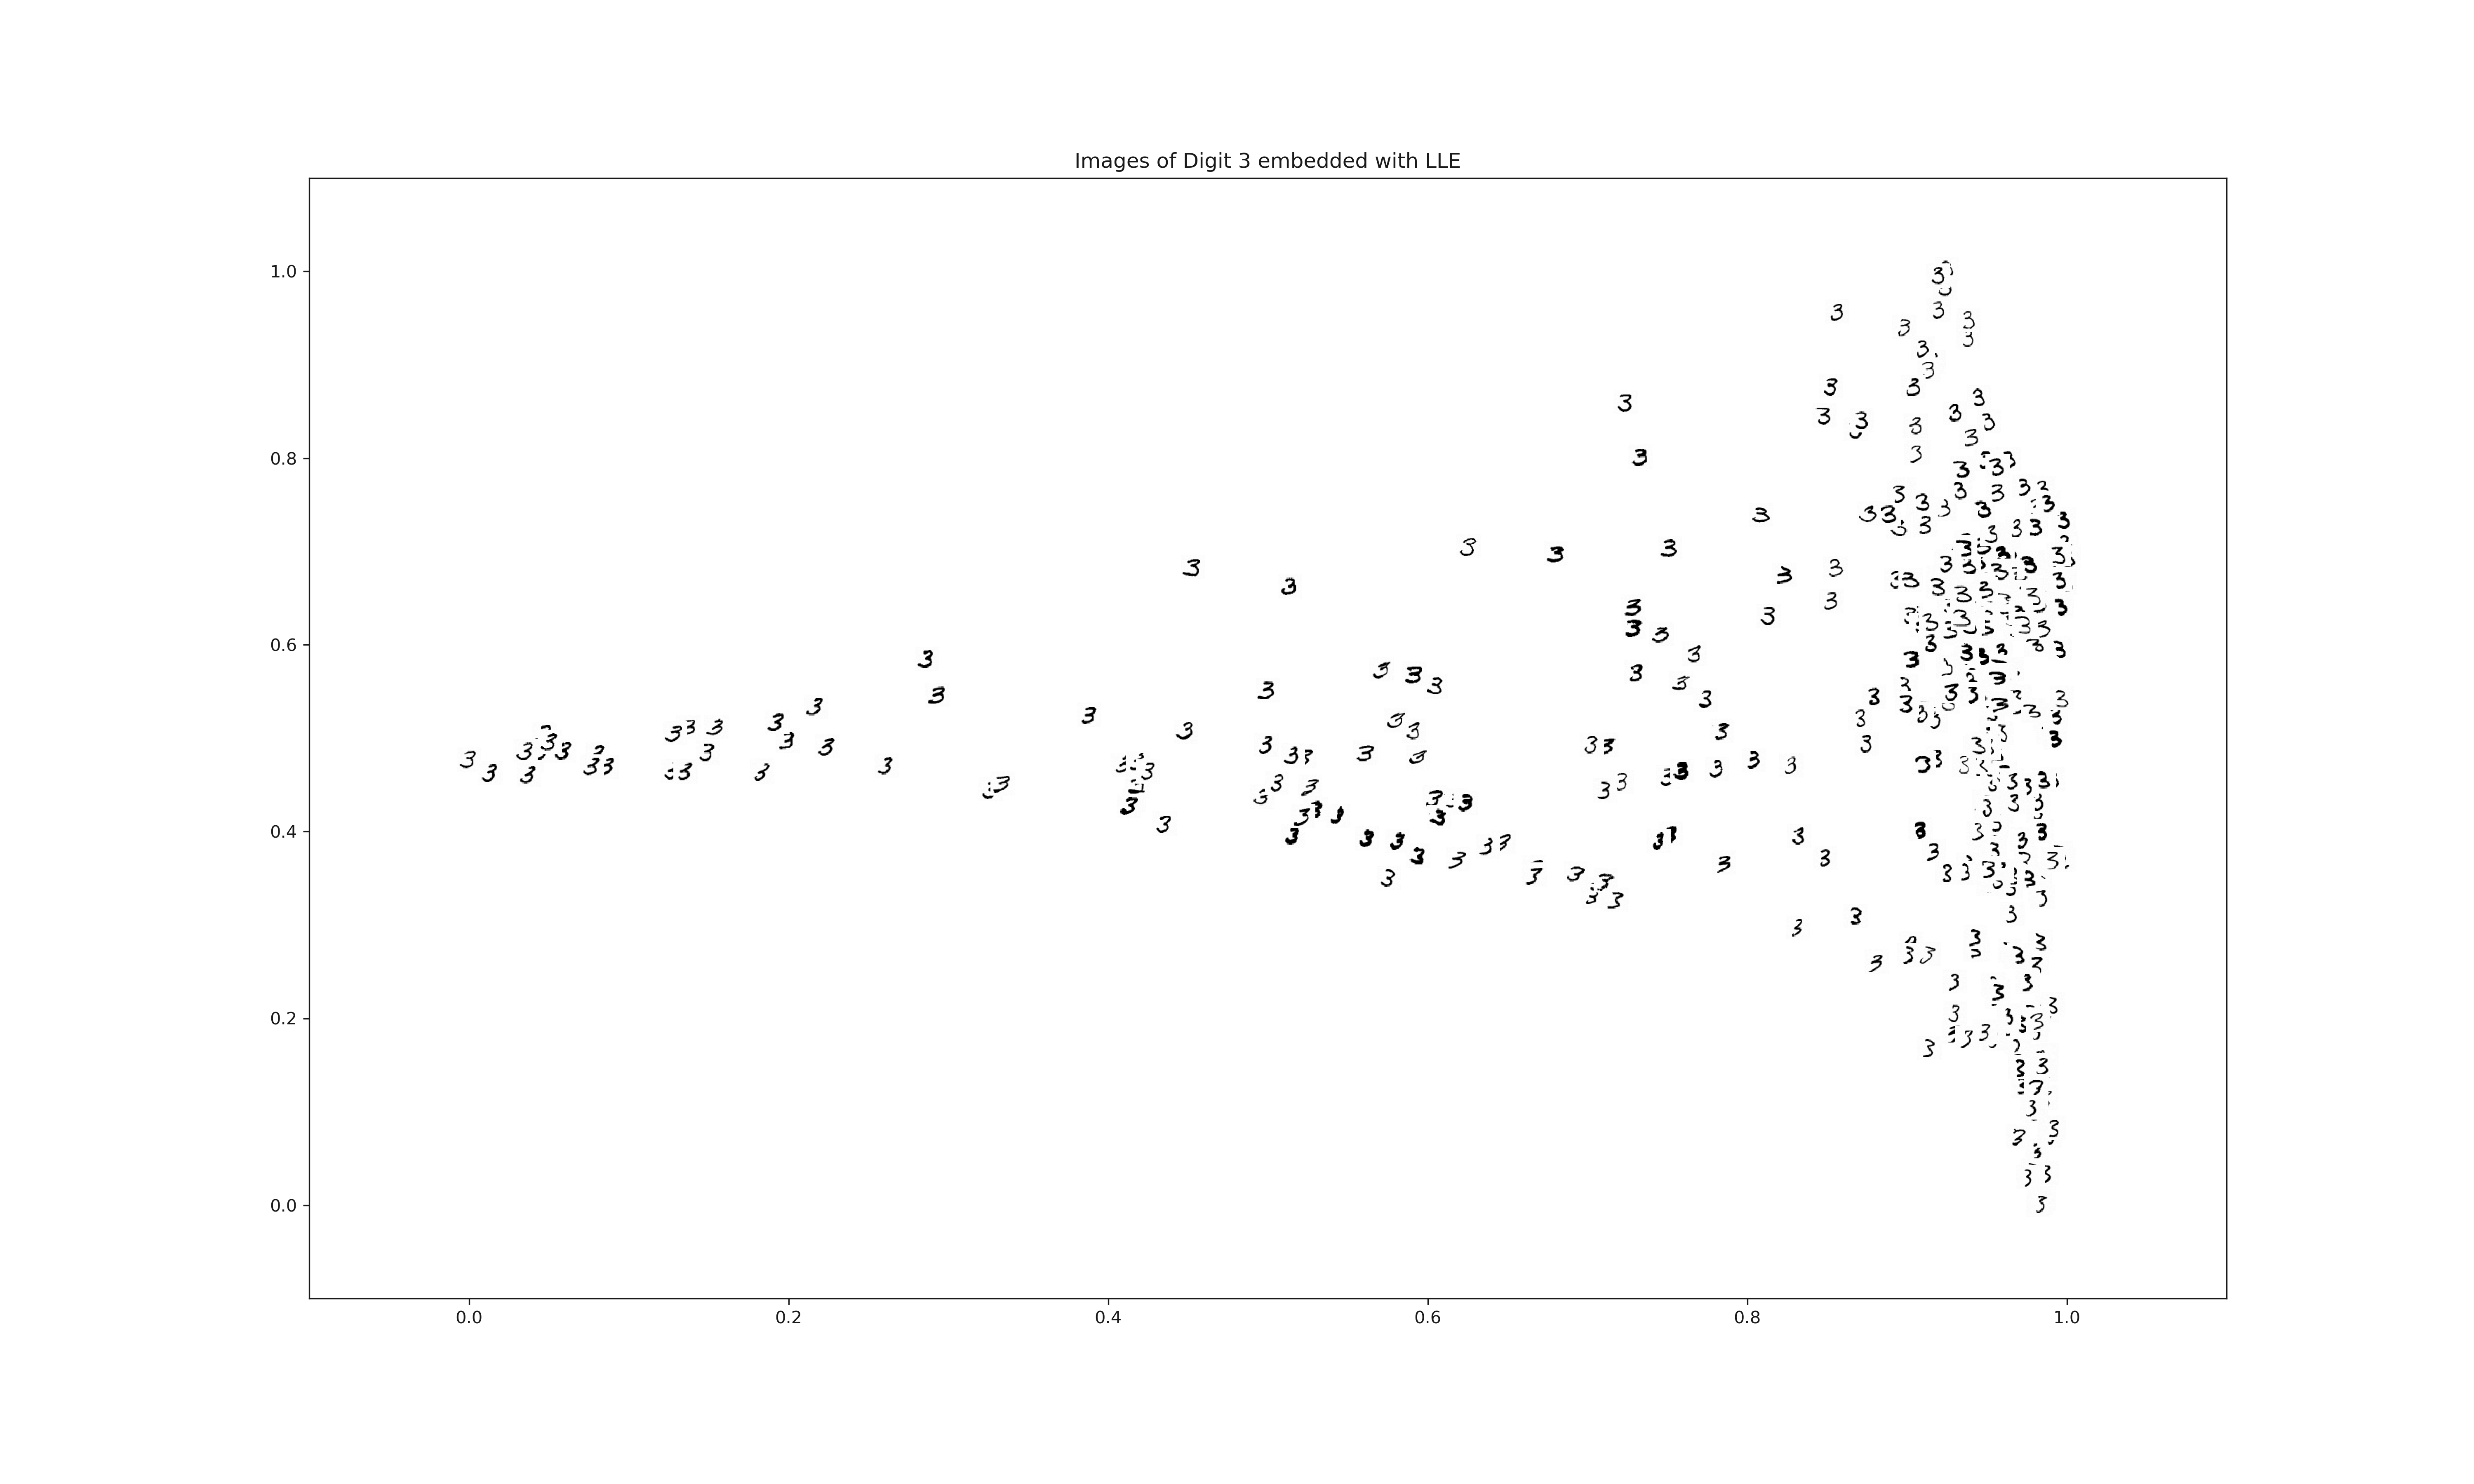
\includegraphics[width=\textwidth]{assignment1/3-1-LLEembedding.png}
\caption{\label{fig:fig9}Images of digit "3" embedded with LLE}
\end{figure}



\clearpage{}
\subsection{Applying ISOMAP to the images of digit '3' only}

The result gives  an idea of the variety of forms that the digit "3" can take within the dataset. The data lies from left to right in  the projected space, which appears to trace the orientation of the digit.We can see that going from left to right of the graph, the digits generally go from tilted to the right to tilted to the left, as you move towards the middle and top center of the plot, you find three's that are partially written or look like other digits and some digits with weak strokes. The projection lets us identify outliers that have data issues: for example, pieces of the neighboring digits that snuck into the extracted images.
Isomap did quite better in mapping the digits both by direction and by thickness. 
Isomap dimensions seem to describe global patterns of the digits: the overall tilt to the right or tilt to the left of the digit from left to right.


Figure~\ref{fig:fig10} .....
\begin{figure}[htb]
 \centering
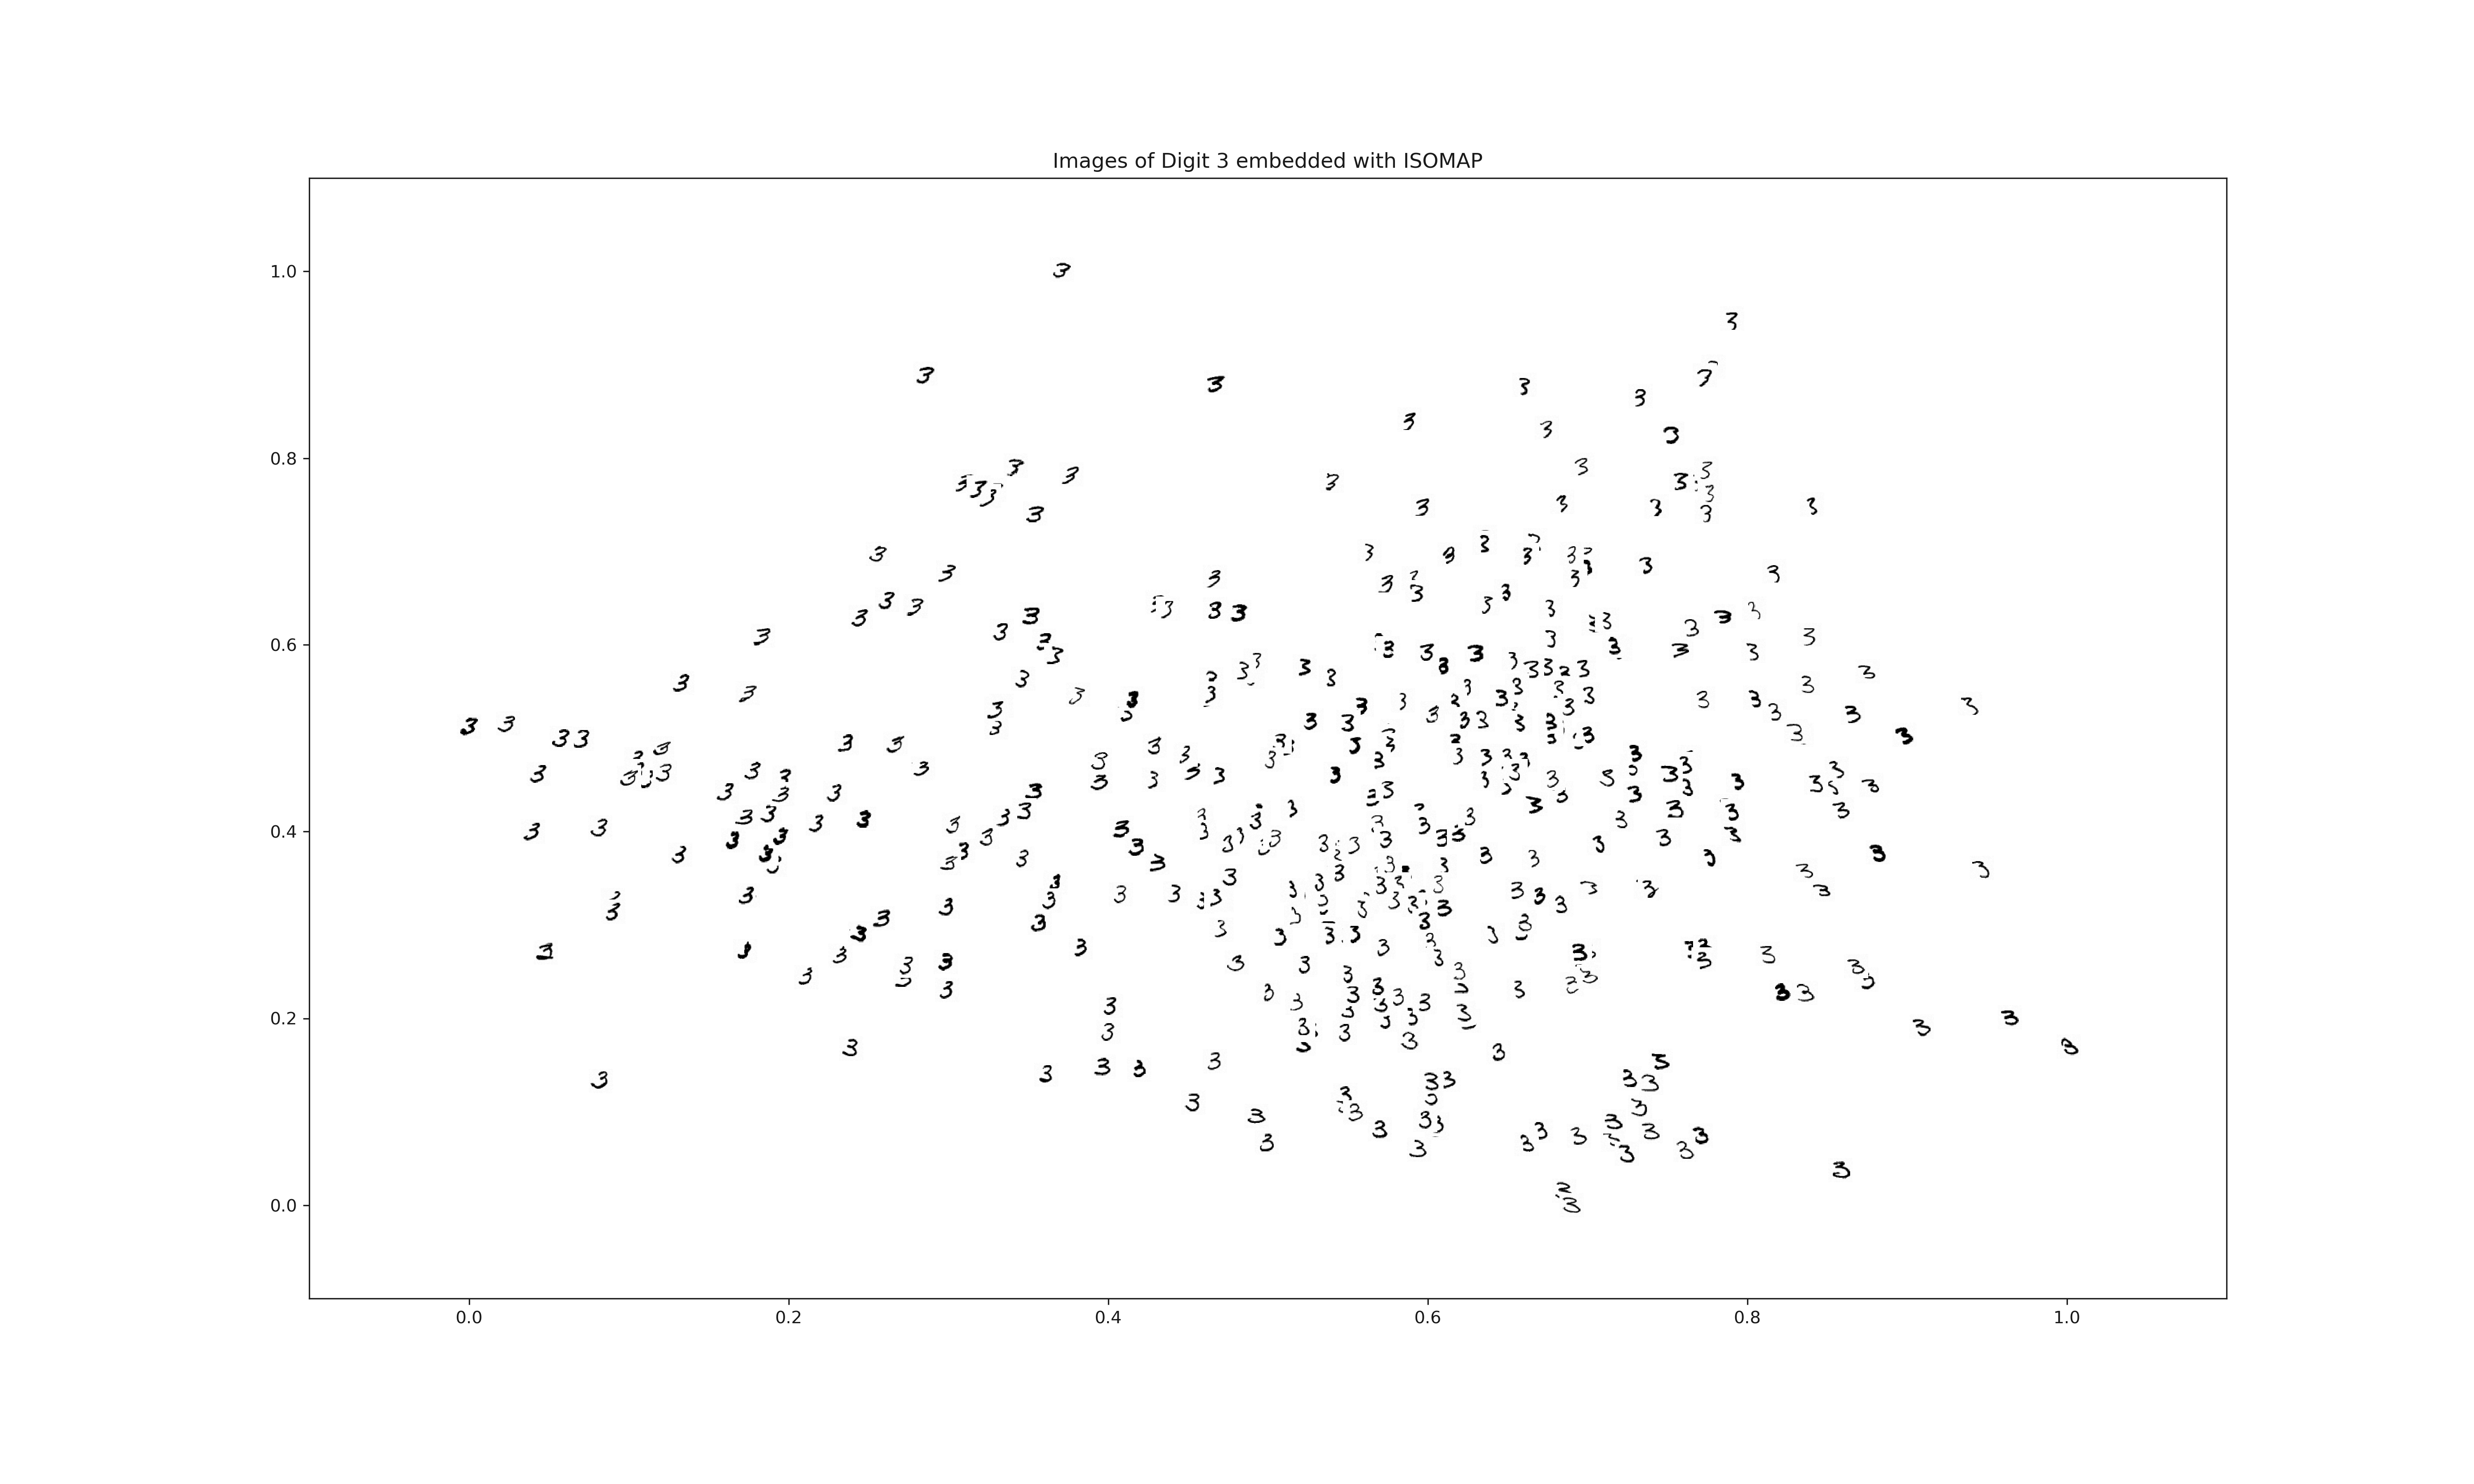
\includegraphics[width=\textwidth]{assignment1/3-2-ISOMAPembedding.png}
\caption{\label{fig:fig10}Images of digit "3" embedded with Isomap}
\end{figure}

\clearpage{}
\subsection{Naive Bayes classifier}

This is the beginning of the subsection.

